\documentclass[1p]{elsarticle_modified}
%\bibliographystyle{elsarticle-num}

%\usepackage[colorlinks]{hyperref}
%\usepackage{abbrmath_seonhwa} %\Abb, \Ascr, \Acal ,\Abf, \Afrak
\usepackage{amsfonts}
\usepackage{amssymb}
\usepackage{amsmath}
\usepackage{amsthm}
\usepackage{scalefnt}
\usepackage{amsbsy}
\usepackage{kotex}
\usepackage{caption}
\usepackage{subfig}
\usepackage{color}
\usepackage{graphicx}
\usepackage{xcolor} %% white, black, red, green, blue, cyan, magenta, yellow
\usepackage{float}
\usepackage{setspace}
\usepackage{hyperref}

\usepackage{tikz}
\usetikzlibrary{arrows}

\usepackage{multirow}
\usepackage{array} % fixed length table
\usepackage{hhline}

%%%%%%%%%%%%%%%%%%%%%
\makeatletter
\renewcommand*\env@matrix[1][\arraystretch]{%
	\edef\arraystretch{#1}%
	\hskip -\arraycolsep
	\let\@ifnextchar\new@ifnextchar
	\array{*\c@MaxMatrixCols c}}
\makeatother %https://tex.stackexchange.com/questions/14071/how-can-i-increase-the-line-spacing-in-a-matrix
%%%%%%%%%%%%%%%

\usepackage[normalem]{ulem}

\newcommand{\msout}[1]{\ifmmode\text{\sout{\ensuremath{#1}}}\else\sout{#1}\fi}
%SOURCE: \msout is \stkout macro in https://tex.stackexchange.com/questions/20609/strikeout-in-math-mode

\newcommand{\cancel}[1]{
	\ifmmode
	{\color{red}\msout{#1}}
	\else
	{\color{red}\sout{#1}}
	\fi
}

\newcommand{\add}[1]{
	{\color{blue}\uwave{#1}}
}

\newcommand{\replace}[2]{
	\ifmmode
	{\color{red}\msout{#1}}{\color{blue}\uwave{#2}}
	\else
	{\color{red}\sout{#1}}{\color{blue}\uwave{#2}}
	\fi
}

\newcommand{\Sol}{\mathcal{S}} %segment
\newcommand{\D}{D} %diagram
\newcommand{\A}{\mathcal{A}} %arc


%%%%%%%%%%%%%%%%%%%%%%%%%%%%%5 test

\def\sl{\operatorname{\textup{SL}}(2,\Cbb)}
\def\psl{\operatorname{\textup{PSL}}(2,\Cbb)}
\def\quan{\mkern 1mu \triangleright \mkern 1mu}

\theoremstyle{definition}
\newtheorem{thm}{Theorem}[section]
\newtheorem{prop}[thm]{Proposition}
\newtheorem{lem}[thm]{Lemma}
\newtheorem{ques}[thm]{Question}
\newtheorem{cor}[thm]{Corollary}
\newtheorem{defn}[thm]{Definition}
\newtheorem{exam}[thm]{Example}
\newtheorem{rmk}[thm]{Remark}
\newtheorem{alg}[thm]{Algorithm}

\newcommand{\I}{\sqrt{-1}}
\begin{document}

%\begin{frontmatter}
%
%\title{Boundary parabolic representations of knots up to 8 crossings}
%
%%% Group authors per affiliation:
%\author{Yunhi Cho} 
%\address{Department of Mathematics, University of Seoul, Seoul, Korea}
%\ead{yhcho@uos.ac.kr}
%
%
%\author{Seonhwa Kim} %\fnref{s_kim}}
%\address{Center for Geometry and Physics, Institute for Basic Science, Pohang, 37673, Korea}
%\ead{ryeona17@ibs.re.kr}
%
%\author{Hyuk Kim}
%\address{Department of Mathematical Sciences, Seoul National University, Seoul 08826, Korea}
%\ead{hyukkim@snu.ac.kr}
%
%\author{Seokbeom Yoon}
%\address{Department of Mathematical Sciences, Seoul National University, Seoul, 08826,  Korea}
%\ead{sbyoon15@snu.ac.kr}
%
%\begin{abstract}
%We find all boundary parabolic representation of knots up to 8 crossings.
%
%\end{abstract}
%\begin{keyword}
%    \MSC[2010] 57M25 
%\end{keyword}
%
%\end{frontmatter}

%\linenumbers
%\tableofcontents
%
\newcommand\colored[1]{\textcolor{white}{\rule[-0.35ex]{0.8em}{1.4ex}}\kern-0.8em\color{red} #1}%
%\newcommand\colored[1]{\textcolor{white}{ #1}\kern-2.17ex	\textcolor{white}{ #1}\kern-1.81ex	\textcolor{white}{ #1}\kern-2.15ex\color{red}#1	}

{\Large $\underline{12n_{0876}~(K12n_{0876})}$}

\setlength{\tabcolsep}{10pt}
\renewcommand{\arraystretch}{1.6}
\vspace{1cm}\begin{tabular}{m{100pt}>{\centering\arraybackslash}m{274pt}}
\multirow{5}{120pt}{
	\centering
	\includegraphics[width=112pt]{../../../GIT/diagram.site/Diagrams/png/2965_12n_0876.png}\\
\ \ \ A knot diagram\footnotemark}&
\allowdisplaybreaks
\textbf{Linearized knot diagam} \\
\cline{2-2}
 &
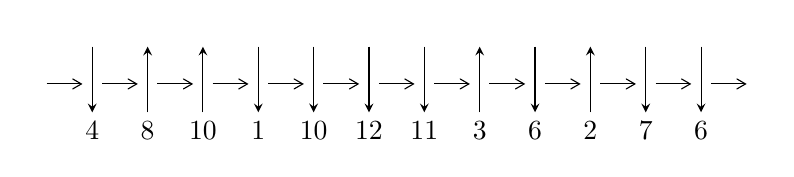
\begin{tikzpicture}[x=20pt, y=17pt]
	% nodes
	\node (C0) at (0, 0) {};
	\node (C1) at (1, 0) {};
	\node (C1U) at (1, +1) {};
	\node (C1D) at (1, -1) {4};

	\node (C2) at (2, 0) {};
	\node (C2U) at (2, +1) {};
	\node (C2D) at (2, -1) {8};

	\node (C3) at (3, 0) {};
	\node (C3U) at (3, +1) {};
	\node (C3D) at (3, -1) {10};

	\node (C4) at (4, 0) {};
	\node (C4U) at (4, +1) {};
	\node (C4D) at (4, -1) {1};

	\node (C5) at (5, 0) {};
	\node (C5U) at (5, +1) {};
	\node (C5D) at (5, -1) {10};

	\node (C6) at (6, 0) {};
	\node (C6U) at (6, +1) {};
	\node (C6D) at (6, -1) {12};

	\node (C7) at (7, 0) {};
	\node (C7U) at (7, +1) {};
	\node (C7D) at (7, -1) {11};

	\node (C8) at (8, 0) {};
	\node (C8U) at (8, +1) {};
	\node (C8D) at (8, -1) {3};

	\node (C9) at (9, 0) {};
	\node (C9U) at (9, +1) {};
	\node (C9D) at (9, -1) {6};

	\node (C10) at (10, 0) {};
	\node (C10U) at (10, +1) {};
	\node (C10D) at (10, -1) {2};

	\node (C11) at (11, 0) {};
	\node (C11U) at (11, +1) {};
	\node (C11D) at (11, -1) {7};

	\node (C12) at (12, 0) {};
	\node (C12U) at (12, +1) {};
	\node (C12D) at (12, -1) {6};
	\node (C13) at (13, 0) {};

	% arrows
	\draw[->,>={angle 60}]
	(C0) edge (C1) (C1) edge (C2) (C2) edge (C3) (C3) edge (C4) (C4) edge (C5) (C5) edge (C6) (C6) edge (C7) (C7) edge (C8) (C8) edge (C9) (C9) edge (C10) (C10) edge (C11) (C11) edge (C12) (C12) edge (C13) ;	\draw[->,>=stealth]
	(C1U) edge (C1D) (C2D) edge (C2U) (C3D) edge (C3U) (C4U) edge (C4D) (C5U) edge (C5D) (C6U) edge (C6D) (C7U) edge (C7D) (C8D) edge (C8U) (C9U) edge (C9D) (C10D) edge (C10U) (C11U) edge (C11D) (C12U) edge (C12D) ;
	\end{tikzpicture} \\
\hhline{~~} \\& 
\textbf{Solving Sequence} \\ \cline{2-2} 
 &
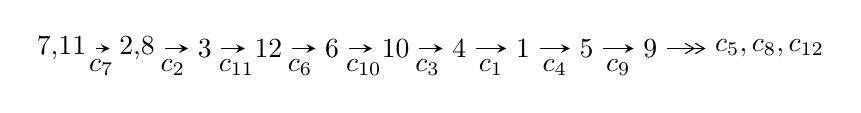
\begin{tikzpicture}[x=23pt, y=7pt]
	% node
	\node (A0) at (-1/8, 0) {7,11};
	\node (A1) at (17/16, 0) {2,8};
	\node (A2) at (17/8, 0) {3};
	\node (A3) at (25/8, 0) {12};
	\node (A4) at (33/8, 0) {6};
	\node (A5) at (41/8, 0) {10};
	\node (A6) at (49/8, 0) {4};
	\node (A7) at (57/8, 0) {1};
	\node (A8) at (65/8, 0) {5};
	\node (A9) at (73/8, 0) {9};
	\node (C1) at (1/2, -1) {$c_{7}$};
	\node (C2) at (13/8, -1) {$c_{2}$};
	\node (C3) at (21/8, -1) {$c_{11}$};
	\node (C4) at (29/8, -1) {$c_{6}$};
	\node (C5) at (37/8, -1) {$c_{10}$};
	\node (C6) at (45/8, -1) {$c_{3}$};
	\node (C7) at (53/8, -1) {$c_{1}$};
	\node (C8) at (61/8, -1) {$c_{4}$};
	\node (C9) at (69/8, -1) {$c_{9}$};
	\node (A10) at (11, 0) {$c_{5},c_{8},c_{12}$};

	% edge
	\draw[->,>=stealth]	
	(A0) edge (A1) (A1) edge (A2) (A2) edge (A3) (A3) edge (A4) (A4) edge (A5) (A5) edge (A6) (A6) edge (A7) (A7) edge (A8) (A8) edge (A9) ;
	\draw[->>,>={angle 60}]	
	(A9) edge (A10);
\end{tikzpicture} \\ 

\end{tabular} \\

\footnotetext{
The image of knot diagram is generated by the software ``\textbf{Draw programme}" developed by Andrew Bartholomew(\url{http://www.layer8.co.uk/maths/draw/index.htm\#Running-draw}), where we modified some parts for our purpose(\url{https://github.com/CATsTAILs/LinksPainter}).
}\phantom \\ \newline 
\centering \textbf{Ideals for irreducible components\footnotemark of $X_{\text{par}}$} 
 
\begin{align*}
I^u_{1}&=\langle 
5 u^{19}-38 u^{18}+\cdots+4 b-40,\;-4 u^{19}+33 u^{18}+\cdots+4 a+38,\;u^{20}-8 u^{19}+\cdots-84 u+8\rangle \\
I^u_{2}&=\langle 
6 a^5 u^3+8 a^4 u^3+\cdots+2 a-2,\;-2 a^4 u^3+a^3 u^3+\cdots+15 a+9,\;u^4+u^3+3 u^2+2 u+1\rangle \\
I^u_{3}&=\langle 
- u^{12}- u^{11}-8 u^{10}-8 u^9-23 u^8-23 u^7-28 u^6-27 u^5-11 u^4-10 u^3+2 u^2+b,\\
\phantom{I^u_{3}}&\phantom{= \langle  }- u^{10}-8 u^8-23 u^6-28 u^4+u^3-12 u^2+a+2 u,\\
\phantom{I^u_{3}}&\phantom{= \langle  }u^{14}+10 u^{12}+39 u^{10}+74 u^8-2 u^7+68 u^6-9 u^5+24 u^4-11 u^3-2 u+1\rangle \\
I^u_{4}&=\langle 
u^2+b+2 u+2,\;- u^3- u^2+a-3 u-2,\;u^4+u^3+3 u^2+2 u+1\rangle \\
I^u_{5}&=\langle 
- u^3- u^2+b-2 u-1,\;2 u^3+2 u^2+a+5 u+3,\;u^4+u^3+3 u^2+2 u+1\rangle \\
I^u_{6}&=\langle 
b+u-1,\;2 a- u+1,\;u^2- u+2\rangle \\
\\
\end{align*}
\raggedright * 6 irreducible components of $\dim_{\mathbb{C}}=0$, with total 68 representations.\\
\footnotetext{All coefficients of polynomials are rational numbers. But the coefficients are sometimes approximated in decimal forms when there is not enough margin.}
\newpage
\renewcommand{\arraystretch}{1}
\centering \section*{I. $I^u_{1}= \langle 5 u^{19}-38 u^{18}+\cdots+4 b-40,\;-4 u^{19}+33 u^{18}+\cdots+4 a+38,\;u^{20}-8 u^{19}+\cdots-84 u+8 \rangle$}
\flushleft \textbf{(i) Arc colorings}\\
\begin{tabular}{m{7pt} m{180pt} m{7pt} m{180pt} }
\flushright $a_{7}=$&$\begin{pmatrix}1\\0\end{pmatrix}$ \\
\flushright $a_{11}=$&$\begin{pmatrix}0\\u\end{pmatrix}$ \\
\flushright $a_{2}=$&$\begin{pmatrix}u^{19}-\frac{33}{4} u^{18}+\cdots+\frac{401}{4} u-\frac{19}{2}\\-\frac{5}{4} u^{19}+\frac{19}{2} u^{18}+\cdots-\frac{207}{2} u+10\end{pmatrix}$ \\
\flushright $a_{8}=$&$\begin{pmatrix}1\\u^2\end{pmatrix}$ \\
\flushright $a_{3}=$&$\begin{pmatrix}\frac{5}{4} u^{19}-\frac{35}{4} u^{18}+\cdots+\frac{103}{4} u-\frac{3}{2}\\\frac{3}{4} u^{19}-\frac{9}{2} u^{18}+\cdots+\frac{41}{2} u-2\end{pmatrix}$ \\
\flushright $a_{12}=$&$\begin{pmatrix}- u\\u\end{pmatrix}$ \\
\flushright $a_{6}=$&$\begin{pmatrix}u^2+1\\- u^2\end{pmatrix}$ \\
\flushright $a_{10}=$&$\begin{pmatrix}- u^{19}+\frac{13}{2} u^{18}+\cdots-10 u+\frac{1}{2}\\\frac{1}{2} u^{18}-3 u^{17}+\cdots-\frac{67}{2} u+4\end{pmatrix}$ \\
\flushright $a_{4}=$&$\begin{pmatrix}\frac{7}{4} u^{19}-\frac{51}{4} u^{18}+\cdots+\frac{633}{4} u-17\\-\frac{3}{4} u^{19}+6 u^{18}+\cdots-161 u+18\end{pmatrix}$ \\
\flushright $a_{1}=$&$\begin{pmatrix}- u^3-2 u\\u^3+u\end{pmatrix}$ \\
\flushright $a_{5}=$&$\begin{pmatrix}-\frac{9}{4} u^{19}+\frac{69}{4} u^{18}+\cdots-\frac{1071}{4} u+27\\\frac{5}{4} u^{19}-9 u^{18}+\cdots+86 u-8\end{pmatrix}$ \\
\flushright $a_{9}=$&$\begin{pmatrix}-\frac{1}{2} u^{19}+4 u^{18}+\cdots-\frac{147}{2} u+\frac{17}{2}\\- u^{19}+\frac{15}{2} u^{18}+\cdots-\frac{159}{2} u+8\end{pmatrix}$\\&\end{tabular}
\flushleft \textbf{(ii) Obstruction class $= -1$}\\~\\
\flushleft \textbf{(iii) Cusp Shapes $= u^{19}-8 u^{18}+42 u^{17}-163 u^{16}+506 u^{15}-1312 u^{14}+2893 u^{13}-5517 u^{12}+9157 u^{11}-13296 u^{10}+16896 u^9-18758 u^8+18092 u^7-15031 u^6+10601 u^5-6223 u^4+2945 u^3-1076 u^2+282 u-46$}\\~\\
\newpage\renewcommand{\arraystretch}{1}
\flushleft \textbf{(iv) u-Polynomials at the component}\newline \\
\begin{tabular}{m{50pt}|m{274pt}}
Crossings & \hspace{64pt}u-Polynomials at each crossing \\
\hline $$\begin{aligned}c_{1},c_{4}\end{aligned}$$&$\begin{aligned}
&u^{20}-11 u^{19}+\cdots-44 u+8
\end{aligned}$\\
\hline $$\begin{aligned}c_{2},c_{8},c_{10}\end{aligned}$$&$\begin{aligned}
&u^{20}-3 u^{19}+\cdots-3 u+1
\end{aligned}$\\
\hline $$\begin{aligned}c_{3}\end{aligned}$$&$\begin{aligned}
&u^{20}+u^{19}+\cdots+9 u^2+1
\end{aligned}$\\
\hline $$\begin{aligned}c_{5},c_{9}\end{aligned}$$&$\begin{aligned}
&u^{20}+3 u^{19}+\cdots+4 u+1
\end{aligned}$\\
\hline $$\begin{aligned}c_{6},c_{7},c_{11}\\c_{12}\end{aligned}$$&$\begin{aligned}
&u^{20}+8 u^{19}+\cdots+84 u+8
\end{aligned}$\\
\hline
\end{tabular}\\~\\
\newpage\renewcommand{\arraystretch}{1}
\flushleft \textbf{(v) Riley Polynomials at the component}\newline \\
\begin{tabular}{m{50pt}|m{274pt}}
Crossings & \hspace{64pt}Riley Polynomials at each crossing \\
\hline $$\begin{aligned}c_{1},c_{4}\end{aligned}$$&$\begin{aligned}
&y^{20}+9 y^{19}+\cdots+48 y+64
\end{aligned}$\\
\hline $$\begin{aligned}c_{2},c_{8},c_{10}\end{aligned}$$&$\begin{aligned}
&y^{20}-15 y^{19}+\cdots- y+1
\end{aligned}$\\
\hline $$\begin{aligned}c_{3}\end{aligned}$$&$\begin{aligned}
&y^{20}+9 y^{19}+\cdots+18 y+1
\end{aligned}$\\
\hline $$\begin{aligned}c_{5},c_{9}\end{aligned}$$&$\begin{aligned}
&y^{20}-19 y^{19}+\cdots+6 y+1
\end{aligned}$\\
\hline $$\begin{aligned}c_{6},c_{7},c_{11}\\c_{12}\end{aligned}$$&$\begin{aligned}
&y^{20}+22 y^{19}+\cdots+240 y+64
\end{aligned}$\\
\hline
\end{tabular}\\~\\
\newpage\flushleft \textbf{(vi) Complex Volumes and Cusp Shapes}
$$\begin{array}{c|c|c}  
\text{Solutions to }I^u_{1}& \I (\text{vol} + \sqrt{-1}CS) & \text{Cusp shape}\\
 \hline 
\begin{aligned}
u &= \phantom{-}0.615618 + 0.809804 I \\
a &= \phantom{-}0.149188 - 1.170140 I \\
b &= \phantom{-}0.085977 + 1.072180 I\end{aligned}
 & -0.57301 - 3.95011 I & -2.11978 + 4.63331 I \\ \hline\begin{aligned}
u &= \phantom{-}0.615618 - 0.809804 I \\
a &= \phantom{-}0.149188 + 1.170140 I \\
b &= \phantom{-}0.085977 - 1.072180 I\end{aligned}
 & -0.57301 + 3.95011 I & -2.11978 - 4.63331 I \\ \hline\begin{aligned}
u &= \phantom{-}0.931383 + 0.280268 I \\
a &= \phantom{-}1.201130 - 0.003287 I \\
b &= -0.170316 + 0.290909 I\end{aligned}
 & -0.03598 + 5.05200 I & -0.41236 - 3.99248 I \\ \hline\begin{aligned}
u &= \phantom{-}0.931383 - 0.280268 I \\
a &= \phantom{-}1.201130 + 0.003287 I \\
b &= -0.170316 - 0.290909 I\end{aligned}
 & -0.03598 - 5.05200 I & -0.41236 + 3.99248 I \\ \hline\begin{aligned}
u &= \phantom{-}0.746449 + 0.775861 I \\
a &= -0.471110 + 1.236680 I \\
b &= -0.100180 - 1.158660 I\end{aligned}
 & \phantom{-}1.47378 - 10.55160 I & \phantom{-}0.34887 + 7.91165 I \\ \hline\begin{aligned}
u &= \phantom{-}0.746449 - 0.775861 I \\
a &= -0.471110 - 1.236680 I \\
b &= -0.100180 + 1.158660 I\end{aligned}
 & \phantom{-}1.47378 + 10.55160 I & \phantom{-}0.34887 - 7.91165 I \\ \hline\begin{aligned}
u &= \phantom{-}0.733781 + 0.211411 I \\
a &= -1.008810 - 0.357032 I \\
b &= \phantom{-}0.277449 - 0.014017 I\end{aligned}
 & -2.40729 - 0.59322 I & -4.18556 - 0.45547 I \\ \hline\begin{aligned}
u &= \phantom{-}0.733781 - 0.211411 I \\
a &= -1.008810 + 0.357032 I \\
b &= \phantom{-}0.277449 + 0.014017 I\end{aligned}
 & -2.40729 + 0.59322 I & -4.18556 + 0.45547 I \\ \hline\begin{aligned}
u &= -0.024618 + 1.249360 I \\
a &= \phantom{-}0.348669 + 0.434224 I \\
b &= \phantom{-}0.033771 - 1.123880 I\end{aligned}
 & \phantom{-}4.75638 - 1.46611 I & \phantom{-}2.62808 + 4.96498 I \\ \hline\begin{aligned}
u &= -0.024618 - 1.249360 I \\
a &= \phantom{-}0.348669 - 0.434224 I \\
b &= \phantom{-}0.033771 + 1.123880 I\end{aligned}
 & \phantom{-}4.75638 + 1.46611 I & \phantom{-}2.62808 - 4.96498 I\\
 \hline 
 \end{array}$$\newpage$$\begin{array}{c|c|c}  
\text{Solutions to }I^u_{1}& \I (\text{vol} + \sqrt{-1}CS) & \text{Cusp shape}\\
 \hline 
\begin{aligned}
u &= \phantom{-}0.259646 + 1.352180 I \\
a &= \phantom{-}0.352486 - 0.235426 I \\
b &= -0.865270 + 0.246592 I\end{aligned}
 & \phantom{-}2.47957 - 4.10039 I & \phantom{-}3.08727 - 0.58697 I \\ \hline\begin{aligned}
u &= \phantom{-}0.259646 - 1.352180 I \\
a &= \phantom{-}0.352486 + 0.235426 I \\
b &= -0.865270 - 0.246592 I\end{aligned}
 & \phantom{-}2.47957 + 4.10039 I & \phantom{-}3.08727 + 0.58697 I \\ \hline\begin{aligned}
u &= \phantom{-}0.240761 + 0.325217 I \\
a &= -0.616636 - 1.071860 I \\
b &= -0.002796 + 0.413272 I\end{aligned}
 & -0.172616 - 0.899774 I & -3.76752 + 7.66615 I \\ \hline\begin{aligned}
u &= \phantom{-}0.240761 - 0.325217 I \\
a &= -0.616636 + 1.071860 I \\
b &= -0.002796 - 0.413272 I\end{aligned}
 & -0.172616 + 0.899774 I & -3.76752 - 7.66615 I \\ \hline\begin{aligned}
u &= \phantom{-}0.23882 + 1.63854 I \\
a &= -0.282035 - 0.978235 I \\
b &= -0.02878 + 3.04561 I\end{aligned}
 & \phantom{-}9.5379 - 14.3084 I & \phantom{-}2.45273 + 7.13980 I \\ \hline\begin{aligned}
u &= \phantom{-}0.23882 - 1.63854 I \\
a &= -0.282035 + 0.978235 I \\
b &= -0.02878 - 3.04561 I\end{aligned}
 & \phantom{-}9.5379 + 14.3084 I & \phantom{-}2.45273 - 7.13980 I \\ \hline\begin{aligned}
u &= \phantom{-}0.19941 + 1.65855 I \\
a &= \phantom{-}0.329642 + 0.850090 I \\
b &= -0.11179 - 2.80281 I\end{aligned}
 & \phantom{-}7.82775 - 7.13457 I & \phantom{-}0.46687 + 4.13636 I \\ \hline\begin{aligned}
u &= \phantom{-}0.19941 - 1.65855 I \\
a &= \phantom{-}0.329642 - 0.850090 I \\
b &= -0.11179 + 2.80281 I\end{aligned}
 & \phantom{-}7.82775 + 7.13457 I & \phantom{-}0.46687 - 4.13636 I \\ \hline\begin{aligned}
u &= \phantom{-}0.05874 + 1.80462 I \\
a &= -0.252521 - 0.599270 I \\
b &= -0.11806 + 2.38692 I\end{aligned}
 & \phantom{-}16.5920 - 2.0882 I & -4.99860 + 4.75350 I \\ \hline\begin{aligned}
u &= \phantom{-}0.05874 - 1.80462 I \\
a &= -0.252521 + 0.599270 I \\
b &= -0.11806 - 2.38692 I\end{aligned}
 & \phantom{-}16.5920 + 2.0882 I & -4.99860 - 4.75350 I\\
 \hline 
 \end{array}$$\newpage\newpage\renewcommand{\arraystretch}{1}
\centering \section*{II. $I^u_{2}= \langle 6 a^5 u^3+8 a^4 u^3+\cdots+2 a-2,\;-2 a^4 u^3+a^3 u^3+\cdots+15 a+9,\;u^4+u^3+3 u^2+2 u+1 \rangle$}
\flushleft \textbf{(i) Arc colorings}\\
\begin{tabular}{m{7pt} m{180pt} m{7pt} m{180pt} }
\flushright $a_{7}=$&$\begin{pmatrix}1\\0\end{pmatrix}$ \\
\flushright $a_{11}=$&$\begin{pmatrix}0\\u\end{pmatrix}$ \\
\flushright $a_{2}=$&$\begin{pmatrix}a\\-3 a^5 u^3-4 a^4 u^3+\cdots- a+1\end{pmatrix}$ \\
\flushright $a_{8}=$&$\begin{pmatrix}1\\u^2\end{pmatrix}$ \\
\flushright $a_{3}=$&$\begin{pmatrix}-3 a^5 u^3-4 a^4 u^3+\cdots-\frac{5}{2} a^2+1\\5 a^5 u^3+7 a^4 u^3+\cdots- a-2\end{pmatrix}$ \\
\flushright $a_{12}=$&$\begin{pmatrix}- u\\u\end{pmatrix}$ \\
\flushright $a_{6}=$&$\begin{pmatrix}u^2+1\\- u^2\end{pmatrix}$ \\
\flushright $a_{10}=$&$\begin{pmatrix}- a^2 u\\4 a^5 u^3+\frac{11}{2} a^4 u^3+\cdots-\frac{1}{2} a-\frac{1}{2}\end{pmatrix}$ \\
\flushright $a_{4}=$&$\begin{pmatrix}2 a^5 u^3+\frac{3}{2} a^4 u^3+\cdots+\frac{5}{2} a-\frac{1}{2}\\-3 a^5 u^3+\frac{3}{2} a^4 u^3+\cdots-\frac{17}{2} a-\frac{1}{2}\end{pmatrix}$ \\
\flushright $a_{1}=$&$\begin{pmatrix}- u^3-2 u\\u^3+u\end{pmatrix}$ \\
\flushright $a_{5}=$&$\begin{pmatrix}2 a^5 u^3+a^4 u^3+\cdots+4 a-1\\- a^5 u^3+\frac{11}{2} a^4 u^3+\cdots-12 a-\frac{5}{2}\end{pmatrix}$ \\
\flushright $a_{9}=$&$\begin{pmatrix}\frac{17}{2} a^5 u^3+\frac{27}{2} a^4 u^3+\cdots-4 a-4\\-\frac{21}{2} a^5 u^3-17 a^4 u^3+\cdots+5 a+\frac{15}{2}\end{pmatrix}$\\&\end{tabular}
\flushleft \textbf{(ii) Obstruction class $= -1$}\\~\\
\flushleft \textbf{(iii) Cusp Shapes $= -4 a^5 u^3+6 a^5 u^2-8 a^4 u^3+6 a^5 u+8 a^4 u^2-6 a^3 u^3+4 a^5+8 a^4 u+24 a^3 u^2-4 u^3 a^2+6 a^4+20 a^3 u+30 a^2 u^2+12 a^3+26 a^2 u+20 u^2 a+2 u^3+14 a^2+14 a u+12 u^2+6 a+2 u$}\\~\\
\newpage\renewcommand{\arraystretch}{1}
\flushleft \textbf{(iv) u-Polynomials at the component}\newline \\
\begin{tabular}{m{50pt}|m{274pt}}
Crossings & \hspace{64pt}u-Polynomials at each crossing \\
\hline $$\begin{aligned}c_{1},c_{4}\end{aligned}$$&$\begin{aligned}
&(u^4+u^3+u^2+1)^6
\end{aligned}$\\
\hline $$\begin{aligned}c_{2},c_{8},c_{10}\end{aligned}$$&$\begin{aligned}
&u^{24}- u^{23}+\cdots-1188 u+328
\end{aligned}$\\
\hline $$\begin{aligned}c_{3}\end{aligned}$$&$\begin{aligned}
&u^{24}+3 u^{23}+\cdots-3996 u+648
\end{aligned}$\\
\hline $$\begin{aligned}c_{5},c_{9}\end{aligned}$$&$\begin{aligned}
&u^{24}+5 u^{23}+\cdots+168 u+8
\end{aligned}$\\
\hline $$\begin{aligned}c_{6},c_{7},c_{11}\\c_{12}\end{aligned}$$&$\begin{aligned}
&(u^4- u^3+3 u^2-2 u+1)^6
\end{aligned}$\\
\hline
\end{tabular}\\~\\
\newpage\renewcommand{\arraystretch}{1}
\flushleft \textbf{(v) Riley Polynomials at the component}\newline \\
\begin{tabular}{m{50pt}|m{274pt}}
Crossings & \hspace{64pt}Riley Polynomials at each crossing \\
\hline $$\begin{aligned}c_{1},c_{4}\end{aligned}$$&$\begin{aligned}
&(y^4+y^3+3 y^2+2 y+1)^6
\end{aligned}$\\
\hline $$\begin{aligned}c_{2},c_{8},c_{10}\end{aligned}$$&$\begin{aligned}
&y^{24}-15 y^{23}+\cdots-453584 y+107584
\end{aligned}$\\
\hline $$\begin{aligned}c_{3}\end{aligned}$$&$\begin{aligned}
&y^{24}-3 y^{23}+\cdots-5750352 y+419904
\end{aligned}$\\
\hline $$\begin{aligned}c_{5},c_{9}\end{aligned}$$&$\begin{aligned}
&y^{24}-7 y^{23}+\cdots-7776 y+64
\end{aligned}$\\
\hline $$\begin{aligned}c_{6},c_{7},c_{11}\\c_{12}\end{aligned}$$&$\begin{aligned}
&(y^4+5 y^3+7 y^2+2 y+1)^6
\end{aligned}$\\
\hline
\end{tabular}\\~\\
\newpage\flushleft \textbf{(vi) Complex Volumes and Cusp Shapes}
$$\begin{array}{c|c|c}  
\text{Solutions to }I^u_{2}& \I (\text{vol} + \sqrt{-1}CS) & \text{Cusp shape}\\
 \hline 
\begin{aligned}
u &= -0.395123 + 0.506844 I \\
a &= \phantom{-}0.103728 - 1.096500 I \\
b &= -1.09009 + 1.02540 I\end{aligned}
 & -2.06694 - 1.74886 I & -1.65348 - 2.34394 I \\ \hline\begin{aligned}
u &= -0.395123 + 0.506844 I \\
a &= \phantom{-}0.16699 + 1.52687 I \\
b &= \phantom{-}0.83629 - 1.36113 I\end{aligned}
 & -2.06694 + 4.57907 I & -1.65348 - 7.47354 I \\ \hline\begin{aligned}
u &= -0.395123 + 0.506844 I \\
a &= -1.78646 + 0.12907 I \\
b &= -0.283051 + 0.216704 I\end{aligned}
 & -2.06694 - 1.74886 I & -1.65348 - 2.34394 I \\ \hline\begin{aligned}
u &= -0.395123 + 0.506844 I \\
a &= \phantom{-}1.63057 - 0.79455 I \\
b &= \phantom{-}0.357314 - 0.054366 I\end{aligned}
 & -2.06694 + 4.57907 I & -1.65348 - 7.47354 I \\ \hline\begin{aligned}
u &= -0.395123 + 0.506844 I \\
a &= -0.39246 - 1.95028 I \\
b &= \phantom{-}0.628050 + 0.462471 I\end{aligned}
 & \phantom{-}4.93480 + 2.83021 I & \phantom{-}2.00000 - 9.81749 I \\ \hline\begin{aligned}
u &= -0.395123 + 0.506844 I \\
a &= \phantom{-}1.17687 + 1.78486 I \\
b &= -0.547258 - 1.222920 I\end{aligned}
 & \phantom{-}4.93480 + 2.83021 I & \phantom{-}2.00000 - 9.81749 I \\ \hline\begin{aligned}
u &= -0.395123 - 0.506844 I \\
a &= \phantom{-}0.103728 + 1.096500 I \\
b &= -1.09009 - 1.02540 I\end{aligned}
 & -2.06694 + 1.74886 I & -1.65348 + 2.34394 I \\ \hline\begin{aligned}
u &= -0.395123 - 0.506844 I \\
a &= \phantom{-}0.16699 - 1.52687 I \\
b &= \phantom{-}0.83629 + 1.36113 I\end{aligned}
 & -2.06694 - 4.57907 I & -1.65348 + 7.47354 I \\ \hline\begin{aligned}
u &= -0.395123 - 0.506844 I \\
a &= -1.78646 - 0.12907 I \\
b &= -0.283051 - 0.216704 I\end{aligned}
 & -2.06694 + 1.74886 I & -1.65348 + 2.34394 I \\ \hline\begin{aligned}
u &= -0.395123 - 0.506844 I \\
a &= \phantom{-}1.63057 + 0.79455 I \\
b &= \phantom{-}0.357314 + 0.054366 I\end{aligned}
 & -2.06694 - 4.57907 I & -1.65348 + 7.47354 I\\
 \hline 
 \end{array}$$\newpage$$\begin{array}{c|c|c}  
\text{Solutions to }I^u_{2}& \I (\text{vol} + \sqrt{-1}CS) & \text{Cusp shape}\\
 \hline 
\begin{aligned}
u &= -0.395123 - 0.506844 I \\
a &= -0.39246 + 1.95028 I \\
b &= \phantom{-}0.628050 - 0.462471 I\end{aligned}
 & \phantom{-}4.93480 - 2.83021 I & \phantom{-}2.00000 + 9.81749 I \\ \hline\begin{aligned}
u &= -0.395123 - 0.506844 I \\
a &= \phantom{-}1.17687 - 1.78486 I \\
b &= -0.547258 + 1.222920 I\end{aligned}
 & \phantom{-}4.93480 - 2.83021 I & \phantom{-}2.00000 + 9.81749 I \\ \hline\begin{aligned}
u &= -0.10488 + 1.55249 I \\
a &= \phantom{-}0.104373 - 0.975826 I \\
b &= \phantom{-}0.81052 + 3.36343 I\end{aligned}
 & \phantom{-}11.93650 + 4.57907 I & \phantom{-}5.65348 - 7.47354 I \\ \hline\begin{aligned}
u &= -0.10488 + 1.55249 I \\
a &= -1.045950 - 0.024912 I \\
b &= \phantom{-}1.324300 + 0.197152 I\end{aligned}
 & \phantom{-}4.93480 + 6.32793 I & \phantom{-}2.00000 - 5.12960 I \\ \hline\begin{aligned}
u &= -0.10488 + 1.55249 I \\
a &= -0.617508 + 0.929773 I \\
b &= \phantom{-}0.28030 - 2.29404 I\end{aligned}
 & \phantom{-}11.93650 + 4.57907 I & \phantom{-}5.65348 - 7.47354 I \\ \hline\begin{aligned}
u &= -0.10488 + 1.55249 I \\
a &= -0.145302 + 1.200950 I \\
b &= -0.31108 - 3.25723 I\end{aligned}
 & \phantom{-}11.93650 + 1.74886 I & \phantom{-}5.65348 + 2.34394 I \\ \hline\begin{aligned}
u &= -0.10488 + 1.55249 I \\
a &= \phantom{-}0.079320 - 0.763538 I \\
b &= -0.58732 + 3.42729 I\end{aligned}
 & \phantom{-}4.93480 + 6.32793 I & \phantom{-}2.00000 - 5.12960 I \\ \hline\begin{aligned}
u &= -0.10488 + 1.55249 I \\
a &= \phantom{-}0.225836 - 0.692087 I \\
b &= \phantom{-}1.08202 + 1.93847 I\end{aligned}
 & \phantom{-}11.93650 + 1.74886 I & \phantom{-}5.65348 + 2.34394 I \\ \hline\begin{aligned}
u &= -0.10488 - 1.55249 I \\
a &= \phantom{-}0.104373 + 0.975826 I \\
b &= \phantom{-}0.81052 - 3.36343 I\end{aligned}
 & \phantom{-}11.93650 - 4.57907 I & \phantom{-}5.65348 + 7.47354 I \\ \hline\begin{aligned}
u &= -0.10488 - 1.55249 I \\
a &= -1.045950 + 0.024912 I \\
b &= \phantom{-}1.324300 - 0.197152 I\end{aligned}
 & \phantom{-}4.93480 - 6.32793 I & \phantom{-}2.00000 + 5.12960 I\\
 \hline 
 \end{array}$$\newpage$$\begin{array}{c|c|c}  
\text{Solutions to }I^u_{2}& \I (\text{vol} + \sqrt{-1}CS) & \text{Cusp shape}\\
 \hline 
\begin{aligned}
u &= -0.10488 - 1.55249 I \\
a &= -0.617508 - 0.929773 I \\
b &= \phantom{-}0.28030 + 2.29404 I\end{aligned}
 & \phantom{-}11.93650 - 4.57907 I & \phantom{-}5.65348 + 7.47354 I \\ \hline\begin{aligned}
u &= -0.10488 - 1.55249 I \\
a &= -0.145302 - 1.200950 I \\
b &= -0.31108 + 3.25723 I\end{aligned}
 & \phantom{-}11.93650 - 1.74886 I & \phantom{-}5.65348 - 2.34394 I \\ \hline\begin{aligned}
u &= -0.10488 - 1.55249 I \\
a &= \phantom{-}0.079320 + 0.763538 I \\
b &= -0.58732 - 3.42729 I\end{aligned}
 & \phantom{-}4.93480 - 6.32793 I & \phantom{-}2.00000 + 5.12960 I \\ \hline\begin{aligned}
u &= -0.10488 - 1.55249 I \\
a &= \phantom{-}0.225836 + 0.692087 I \\
b &= \phantom{-}1.08202 - 1.93847 I\end{aligned}
 & \phantom{-}11.93650 - 1.74886 I & \phantom{-}5.65348 - 2.34394 I\\
 \hline 
 \end{array}$$\newpage\newpage\renewcommand{\arraystretch}{1}
\centering \section*{III. $I^u_{3}= \langle - u^{12}- u^{11}+\cdots+2 u^2+b,\;- u^{10}-8 u^8+\cdots+a+2 u,\;u^{14}+10 u^{12}+\cdots-2 u+1 \rangle$}
\flushleft \textbf{(i) Arc colorings}\\
\begin{tabular}{m{7pt} m{180pt} m{7pt} m{180pt} }
\flushright $a_{7}=$&$\begin{pmatrix}1\\0\end{pmatrix}$ \\
\flushright $a_{11}=$&$\begin{pmatrix}0\\u\end{pmatrix}$ \\
\flushright $a_{2}=$&$\begin{pmatrix}u^{10}+8 u^8+23 u^6+28 u^4- u^3+12 u^2-2 u\\u^{12}+u^{11}+\cdots+10 u^3-2 u^2\end{pmatrix}$ \\
\flushright $a_{8}=$&$\begin{pmatrix}1\\u^2\end{pmatrix}$ \\
\flushright $a_{3}=$&$\begin{pmatrix}u^{11}+u^{10}+\cdots+10 u^2-2 u\\u^{13}+u^{12}+\cdots+10 u^3-2 u^2\end{pmatrix}$ \\
\flushright $a_{12}=$&$\begin{pmatrix}- u\\u\end{pmatrix}$ \\
\flushright $a_{6}=$&$\begin{pmatrix}u^2+1\\- u^2\end{pmatrix}$ \\
\flushright $a_{10}=$&$\begin{pmatrix}- u^{12}-9 u^{10}-31 u^8-51 u^6+2 u^5-40 u^4+7 u^3-12 u^2+6 u\\- u^{13}+u^{12}+\cdots- u+1\end{pmatrix}$ \\
\flushright $a_{4}=$&$\begin{pmatrix}u^{11}+9 u^9+30 u^7+45 u^5- u^4+29 u^3-4 u^2+6 u-3\\u^{10}+7 u^8+17 u^6+16 u^4-2 u^3+4 u^2-3 u\end{pmatrix}$ \\
\flushright $a_{1}=$&$\begin{pmatrix}- u^3-2 u\\u^3+u\end{pmatrix}$ \\
\flushright $a_{5}=$&$\begin{pmatrix}u^9+7 u^7+17 u^5+17 u^3- u^2+6 u-2\\u^{12}+u^{11}+\cdots+2 u^2-4 u\end{pmatrix}$ \\
\flushright $a_{9}=$&$\begin{pmatrix}- u^{13}- u^{12}+\cdots+6 u+1\\u^{12}- u^{11}+\cdots- u+1\end{pmatrix}$\\&\end{tabular}
\flushleft \textbf{(ii) Obstruction class $= 1$}\\~\\
\flushleft \textbf{(iii) Cusp Shapes $= - u^{13}+2 u^{12}-8 u^{11}+17 u^{10}-24 u^9+51 u^8-37 u^7+60 u^6-43 u^5+12 u^4-41 u^3-15 u^2-11 u+6$}\\~\\
\newpage\renewcommand{\arraystretch}{1}
\flushleft \textbf{(iv) u-Polynomials at the component}\newline \\
\begin{tabular}{m{50pt}|m{274pt}}
Crossings & \hspace{64pt}u-Polynomials at each crossing \\
\hline $$\begin{aligned}c_{1}\end{aligned}$$&$\begin{aligned}
&u^{14}-3 u^{13}+\cdots+7 u^2+1
\end{aligned}$\\
\hline $$\begin{aligned}c_{2},c_{10}\end{aligned}$$&$\begin{aligned}
&u^{14}- u^{13}+\cdots- u+1
\end{aligned}$\\
\hline $$\begin{aligned}c_{3}\end{aligned}$$&$\begin{aligned}
&u^{14}- u^{12}+\cdots+22 u+29
\end{aligned}$\\
\hline $$\begin{aligned}c_{4}\end{aligned}$$&$\begin{aligned}
&u^{14}+3 u^{13}+\cdots+7 u^2+1
\end{aligned}$\\
\hline $$\begin{aligned}c_{5}\end{aligned}$$&$\begin{aligned}
&u^{14}+u^{13}+\cdots+4 u^2+1
\end{aligned}$\\
\hline $$\begin{aligned}c_{6},c_{7}\end{aligned}$$&$\begin{aligned}
&u^{14}+10 u^{12}+\cdots-2 u+1
\end{aligned}$\\
\hline $$\begin{aligned}c_{8}\end{aligned}$$&$\begin{aligned}
&u^{14}+u^{13}+\cdots+u+1
\end{aligned}$\\
\hline $$\begin{aligned}c_{9}\end{aligned}$$&$\begin{aligned}
&u^{14}- u^{13}+\cdots+4 u^2+1
\end{aligned}$\\
\hline $$\begin{aligned}c_{11},c_{12}\end{aligned}$$&$\begin{aligned}
&u^{14}+10 u^{12}+\cdots+2 u+1
\end{aligned}$\\
\hline
\end{tabular}\\~\\
\newpage\renewcommand{\arraystretch}{1}
\flushleft \textbf{(v) Riley Polynomials at the component}\newline \\
\begin{tabular}{m{50pt}|m{274pt}}
Crossings & \hspace{64pt}Riley Polynomials at each crossing \\
\hline $$\begin{aligned}c_{1},c_{4}\end{aligned}$$&$\begin{aligned}
&y^{14}+11 y^{13}+\cdots+14 y+1
\end{aligned}$\\
\hline $$\begin{aligned}c_{2},c_{8},c_{10}\end{aligned}$$&$\begin{aligned}
&y^{14}-11 y^{13}+\cdots+5 y+1
\end{aligned}$\\
\hline $$\begin{aligned}c_{3}\end{aligned}$$&$\begin{aligned}
&y^{14}-2 y^{13}+\cdots+1082 y+841
\end{aligned}$\\
\hline $$\begin{aligned}c_{5},c_{9}\end{aligned}$$&$\begin{aligned}
&y^{14}-3 y^{13}+\cdots+8 y+1
\end{aligned}$\\
\hline $$\begin{aligned}c_{6},c_{7},c_{11}\\c_{12}\end{aligned}$$&$\begin{aligned}
&y^{14}+20 y^{13}+\cdots-4 y+1
\end{aligned}$\\
\hline
\end{tabular}\\~\\
\newpage\flushleft \textbf{(vi) Complex Volumes and Cusp Shapes}
$$\begin{array}{c|c|c}  
\text{Solutions to }I^u_{3}& \I (\text{vol} + \sqrt{-1}CS) & \text{Cusp shape}\\
 \hline 
\begin{aligned}
u &= -0.311609 + 0.942763 I \\
a &= \phantom{-}0.291653 + 1.169250 I \\
b &= -0.737119 - 1.186440 I\end{aligned}
 & \phantom{-}7.09672 + 0.19743 I & \phantom{-}7.21171 - 0.40759 I \\ \hline\begin{aligned}
u &= -0.311609 - 0.942763 I \\
a &= \phantom{-}0.291653 - 1.169250 I \\
b &= -0.737119 + 1.186440 I\end{aligned}
 & \phantom{-}7.09672 - 0.19743 I & \phantom{-}7.21171 + 0.40759 I \\ \hline\begin{aligned}
u &= \phantom{-}0.161029 + 1.344040 I \\
a &= \phantom{-}0.433516 + 0.120817 I \\
b &= -0.916757 + 0.574654 I\end{aligned}
 & \phantom{-}2.08475 - 4.90341 I & -1.06931 + 6.62394 I \\ \hline\begin{aligned}
u &= \phantom{-}0.161029 - 1.344040 I \\
a &= \phantom{-}0.433516 - 0.120817 I \\
b &= -0.916757 - 0.574654 I\end{aligned}
 & \phantom{-}2.08475 + 4.90341 I & -1.06931 - 6.62394 I \\ \hline\begin{aligned}
u &= \phantom{-}0.23888 + 1.43943 I \\
a &= -0.435879 + 0.255328 I \\
b &= \phantom{-}0.231007 - 1.380650 I\end{aligned}
 & \phantom{-}3.18169 + 0.60898 I & -3.58539 - 1.80775 I \\ \hline\begin{aligned}
u &= \phantom{-}0.23888 - 1.43943 I \\
a &= -0.435879 - 0.255328 I \\
b &= \phantom{-}0.231007 + 1.380650 I\end{aligned}
 & \phantom{-}3.18169 - 0.60898 I & -3.58539 + 1.80775 I \\ \hline\begin{aligned}
u &= -0.293216 + 0.377036 I \\
a &= -1.27142 - 2.57328 I \\
b &= \phantom{-}0.845482 + 0.700844 I\end{aligned}
 & \phantom{-}5.21647 + 1.94152 I & \phantom{-}5.99803 - 0.90958 I \\ \hline\begin{aligned}
u &= -0.293216 - 0.377036 I \\
a &= -1.27142 + 2.57328 I \\
b &= \phantom{-}0.845482 - 0.700844 I\end{aligned}
 & \phantom{-}5.21647 - 1.94152 I & \phantom{-}5.99803 + 0.90958 I \\ \hline\begin{aligned}
u &= -0.09214 + 1.54037 I \\
a &= -0.305542 + 0.999070 I \\
b &= -0.50480 - 2.83803 I\end{aligned}
 & \phantom{-}11.88620 + 3.33387 I & \phantom{-}5.15657 - 1.10675 I \\ \hline\begin{aligned}
u &= -0.09214 - 1.54037 I \\
a &= -0.305542 - 0.999070 I \\
b &= -0.50480 + 2.83803 I\end{aligned}
 & \phantom{-}11.88620 - 3.33387 I & \phantom{-}5.15657 + 1.10675 I\\
 \hline 
 \end{array}$$\newpage$$\begin{array}{c|c|c}  
\text{Solutions to }I^u_{3}& \I (\text{vol} + \sqrt{-1}CS) & \text{Cusp shape}\\
 \hline 
\begin{aligned}
u &= \phantom{-}0.376292 + 0.105089 I \\
a &= \phantom{-}1.06759 + 1.35883 I \\
b &= \phantom{-}0.290833 + 0.885340 I\end{aligned}
 & -2.11738 + 2.98340 I & -1.73215 - 4.07562 I \\ \hline\begin{aligned}
u &= \phantom{-}0.376292 - 0.105089 I \\
a &= \phantom{-}1.06759 - 1.35883 I \\
b &= \phantom{-}0.290833 - 0.885340 I\end{aligned}
 & -2.11738 - 2.98340 I & -1.73215 + 4.07562 I \\ \hline\begin{aligned}
u &= -0.07924 + 1.76897 I \\
a &= \phantom{-}0.220085 - 0.669149 I \\
b &= \phantom{-}0.29136 + 2.47039 I\end{aligned}
 & \phantom{-}17.0648 + 1.9156 I & \phantom{-}10.52053 + 0.88434 I \\ \hline\begin{aligned}
u &= -0.07924 - 1.76897 I \\
a &= \phantom{-}0.220085 + 0.669149 I \\
b &= \phantom{-}0.29136 - 2.47039 I\end{aligned}
 & \phantom{-}17.0648 - 1.9156 I & \phantom{-}10.52053 - 0.88434 I\\
 \hline 
 \end{array}$$\newpage\newpage\renewcommand{\arraystretch}{1}
\centering \section*{IV. $I^u_{4}= \langle u^2+b+2 u+2,\;- u^3- u^2+a-3 u-2,\;u^4+u^3+3 u^2+2 u+1 \rangle$}
\flushleft \textbf{(i) Arc colorings}\\
\begin{tabular}{m{7pt} m{180pt} m{7pt} m{180pt} }
\flushright $a_{7}=$&$\begin{pmatrix}1\\0\end{pmatrix}$ \\
\flushright $a_{11}=$&$\begin{pmatrix}0\\u\end{pmatrix}$ \\
\flushright $a_{2}=$&$\begin{pmatrix}u^3+u^2+3 u+2\\- u^2-2 u-2\end{pmatrix}$ \\
\flushright $a_{8}=$&$\begin{pmatrix}1\\u^2\end{pmatrix}$ \\
\flushright $a_{3}=$&$\begin{pmatrix}u^3+2 u\\-1\end{pmatrix}$ \\
\flushright $a_{12}=$&$\begin{pmatrix}- u\\u\end{pmatrix}$ \\
\flushright $a_{6}=$&$\begin{pmatrix}u^2+1\\- u^2\end{pmatrix}$ \\
\flushright $a_{10}=$&$\begin{pmatrix}u^3+u^2+3 u+2\\- u^2- u-2\end{pmatrix}$ \\
\flushright $a_{4}=$&$\begin{pmatrix}- u^3-2 u^2-3 u-4\\u^2+2\end{pmatrix}$ \\
\flushright $a_{1}=$&$\begin{pmatrix}- u^3-2 u\\u^3+u\end{pmatrix}$ \\
\flushright $a_{5}=$&$\begin{pmatrix}- u^3-2 u^2-3 u-3\\2 u^2+u+2\end{pmatrix}$ \\
\flushright $a_{9}=$&$\begin{pmatrix}u^3+3 u+1\\- u-2\end{pmatrix}$\\&\end{tabular}
\flushleft \textbf{(ii) Obstruction class $= -1$}\\~\\
\flushleft \textbf{(iii) Cusp Shapes $= 2$}\\~\\
\newpage\renewcommand{\arraystretch}{1}
\flushleft \textbf{(iv) u-Polynomials at the component}\newline \\
\begin{tabular}{m{50pt}|m{274pt}}
Crossings & \hspace{64pt}u-Polynomials at each crossing \\
\hline $$\begin{aligned}c_{1},c_{4}\end{aligned}$$&$\begin{aligned}
&u^4+u^3+u^2+1
\end{aligned}$\\
\hline $$\begin{aligned}c_{2},c_{8}\end{aligned}$$&$\begin{aligned}
&u^4-2 u^3+u^2-3 u+4
\end{aligned}$\\
\hline $$\begin{aligned}c_{3}\end{aligned}$$&$\begin{aligned}
&u^4-3 u^3+u^2+2 u+1
\end{aligned}$\\
\hline $$\begin{aligned}c_{5},c_{9}\end{aligned}$$&$\begin{aligned}
&(u-1)^4
\end{aligned}$\\
\hline $$\begin{aligned}c_{6},c_{7},c_{11}\\c_{12}\end{aligned}$$&$\begin{aligned}
&u^4- u^3+3 u^2-2 u+1
\end{aligned}$\\
\hline $$\begin{aligned}c_{10}\end{aligned}$$&$\begin{aligned}
&(u+1)^4
\end{aligned}$\\
\hline
\end{tabular}\\~\\
\newpage\renewcommand{\arraystretch}{1}
\flushleft \textbf{(v) Riley Polynomials at the component}\newline \\
\begin{tabular}{m{50pt}|m{274pt}}
Crossings & \hspace{64pt}Riley Polynomials at each crossing \\
\hline $$\begin{aligned}c_{1},c_{4}\end{aligned}$$&$\begin{aligned}
&y^4+y^3+3 y^2+2 y+1
\end{aligned}$\\
\hline $$\begin{aligned}c_{2},c_{8}\end{aligned}$$&$\begin{aligned}
&y^4-2 y^3-3 y^2- y+16
\end{aligned}$\\
\hline $$\begin{aligned}c_{3}\end{aligned}$$&$\begin{aligned}
&y^4-7 y^3+15 y^2-2 y+1
\end{aligned}$\\
\hline $$\begin{aligned}c_{5},c_{9},c_{10}\end{aligned}$$&$\begin{aligned}
&(y-1)^4
\end{aligned}$\\
\hline $$\begin{aligned}c_{6},c_{7},c_{11}\\c_{12}\end{aligned}$$&$\begin{aligned}
&y^4+5 y^3+7 y^2+2 y+1
\end{aligned}$\\
\hline
\end{tabular}\\~\\
\newpage\flushleft \textbf{(vi) Complex Volumes and Cusp Shapes}
$$\begin{array}{c|c|c}  
\text{Solutions to }I^u_{4}& \I (\text{vol} + \sqrt{-1}CS) & \text{Cusp shape}\\
 \hline 
\begin{aligned}
u &= -0.395123 + 0.506844 I \\
a &= \phantom{-}0.95668 + 1.22719 I \\
b &= -1.108990 - 0.613156 I\end{aligned}
 & \phantom{-}4.93480\phantom{ +0.000000I} & \phantom{-}2.00000\phantom{ +0.000000I} \\ \hline\begin{aligned}
u &= -0.395123 - 0.506844 I \\
a &= \phantom{-}0.95668 - 1.22719 I \\
b &= -1.108990 + 0.613156 I\end{aligned}
 & \phantom{-}4.93480\phantom{ +0.000000I} & \phantom{-}2.00000\phantom{ +0.000000I} \\ \hline\begin{aligned}
u &= -0.10488 + 1.55249 I \\
a &= \phantom{-}0.043315 + 0.641200 I \\
b &= \phantom{-}0.60898 - 2.77934 I\end{aligned}
 & \phantom{-}4.93480\phantom{ +0.000000I} & \phantom{-}2.00000\phantom{ +0.000000I} \\ \hline\begin{aligned}
u &= -0.10488 - 1.55249 I \\
a &= \phantom{-}0.043315 - 0.641200 I \\
b &= \phantom{-}0.60898 + 2.77934 I\end{aligned}
 & \phantom{-}4.93480\phantom{ +0.000000I} & \phantom{-}2.00000\phantom{ +0.000000I}\\
 \hline 
 \end{array}$$\newpage\newpage\renewcommand{\arraystretch}{1}
\centering \section*{V. $I^u_{5}= \langle - u^3- u^2+b-2 u-1,\;2 u^3+2 u^2+a+5 u+3,\;u^4+u^3+3 u^2+2 u+1 \rangle$}
\flushleft \textbf{(i) Arc colorings}\\
\begin{tabular}{m{7pt} m{180pt} m{7pt} m{180pt} }
\flushright $a_{7}=$&$\begin{pmatrix}1\\0\end{pmatrix}$ \\
\flushright $a_{11}=$&$\begin{pmatrix}0\\u\end{pmatrix}$ \\
\flushright $a_{2}=$&$\begin{pmatrix}-2 u^3-2 u^2-5 u-3\\u^3+u^2+2 u+1\end{pmatrix}$ \\
\flushright $a_{8}=$&$\begin{pmatrix}1\\u^2\end{pmatrix}$ \\
\flushright $a_{3}=$&$\begin{pmatrix}-2 u^3-2 u^2-5 u-2\\u^3+2 u^2+2 u+1\end{pmatrix}$ \\
\flushright $a_{12}=$&$\begin{pmatrix}- u\\u\end{pmatrix}$ \\
\flushright $a_{6}=$&$\begin{pmatrix}u^2+1\\- u^2\end{pmatrix}$ \\
\flushright $a_{10}=$&$\begin{pmatrix}3 u^3+2 u^2+7 u+4\\- u^3- u-1\end{pmatrix}$ \\
\flushright $a_{4}=$&$\begin{pmatrix}- u^3-3 u+1\\u\end{pmatrix}$ \\
\flushright $a_{1}=$&$\begin{pmatrix}- u^3-2 u\\u^3+u\end{pmatrix}$ \\
\flushright $a_{5}=$&$\begin{pmatrix}- u^3-3 u+2\\u^2+2 u\end{pmatrix}$ \\
\flushright $a_{9}=$&$\begin{pmatrix}2 u^3+2 u^2+5 u+3\\- u^3- u^2-2 u-1\end{pmatrix}$\\&\end{tabular}
\flushleft \textbf{(ii) Obstruction class $= -1$}\\~\\
\flushleft \textbf{(iii) Cusp Shapes $= 2$}\\~\\
\newpage\renewcommand{\arraystretch}{1}
\flushleft \textbf{(iv) u-Polynomials at the component}\newline \\
\begin{tabular}{m{50pt}|m{274pt}}
Crossings & \hspace{64pt}u-Polynomials at each crossing \\
\hline $$\begin{aligned}c_{1},c_{4}\end{aligned}$$&$\begin{aligned}
&u^4+u^3+u^2+1
\end{aligned}$\\
\hline $$\begin{aligned}c_{2},c_{8}\end{aligned}$$&$\begin{aligned}
&(u+1)^4
\end{aligned}$\\
\hline $$\begin{aligned}c_{3}\end{aligned}$$&$\begin{aligned}
&u^4+u^3+3 u^2+2 u+1
\end{aligned}$\\
\hline $$\begin{aligned}c_{5},c_{9}\end{aligned}$$&$\begin{aligned}
&u^4+2 u^3+3 u^2+3 u+2
\end{aligned}$\\
\hline $$\begin{aligned}c_{6},c_{7},c_{11}\\c_{12}\end{aligned}$$&$\begin{aligned}
&u^4- u^3+3 u^2-2 u+1
\end{aligned}$\\
\hline $$\begin{aligned}c_{10}\end{aligned}$$&$\begin{aligned}
&u^4-2 u^3+u^2-3 u+4
\end{aligned}$\\
\hline
\end{tabular}\\~\\
\newpage\renewcommand{\arraystretch}{1}
\flushleft \textbf{(v) Riley Polynomials at the component}\newline \\
\begin{tabular}{m{50pt}|m{274pt}}
Crossings & \hspace{64pt}Riley Polynomials at each crossing \\
\hline $$\begin{aligned}c_{1},c_{4}\end{aligned}$$&$\begin{aligned}
&y^4+y^3+3 y^2+2 y+1
\end{aligned}$\\
\hline $$\begin{aligned}c_{2},c_{8}\end{aligned}$$&$\begin{aligned}
&(y-1)^4
\end{aligned}$\\
\hline $$\begin{aligned}c_{3},c_{6},c_{7}\\c_{11},c_{12}\end{aligned}$$&$\begin{aligned}
&y^4+5 y^3+7 y^2+2 y+1
\end{aligned}$\\
\hline $$\begin{aligned}c_{5},c_{9}\end{aligned}$$&$\begin{aligned}
&y^4+2 y^3+y^2+3 y+4
\end{aligned}$\\
\hline $$\begin{aligned}c_{10}\end{aligned}$$&$\begin{aligned}
&y^4-2 y^3-3 y^2- y+16
\end{aligned}$\\
\hline
\end{tabular}\\~\\
\newpage\flushleft \textbf{(vi) Complex Volumes and Cusp Shapes}
$$\begin{array}{c|c|c}  
\text{Solutions to }I^u_{5}& \I (\text{vol} + \sqrt{-1}CS) & \text{Cusp shape}\\
 \hline 
\begin{aligned}
u &= -0.395123 + 0.506844 I \\
a &= -1.30849 - 1.94753 I \\
b &= \phantom{-}0.351808 + 0.720342 I\end{aligned}
 & \phantom{-}4.93480\phantom{ +0.000000I} & \phantom{-}2.00000\phantom{ +0.000000I} \\ \hline\begin{aligned}
u &= -0.395123 - 0.506844 I \\
a &= -1.30849 + 1.94753 I \\
b &= \phantom{-}0.351808 - 0.720342 I\end{aligned}
 & \phantom{-}4.93480\phantom{ +0.000000I} & \phantom{-}2.00000\phantom{ +0.000000I} \\ \hline\begin{aligned}
u &= -0.10488 + 1.55249 I \\
a &= \phantom{-}0.808493 + 0.270093 I \\
b &= -0.851808 - 0.911292 I\end{aligned}
 & \phantom{-}4.93480\phantom{ +0.000000I} & \phantom{-}2.00000\phantom{ +0.000000I} \\ \hline\begin{aligned}
u &= -0.10488 - 1.55249 I \\
a &= \phantom{-}0.808493 - 0.270093 I \\
b &= -0.851808 + 0.911292 I\end{aligned}
 & \phantom{-}4.93480\phantom{ +0.000000I} & \phantom{-}2.00000\phantom{ +0.000000I}\\
 \hline 
 \end{array}$$\newpage\newpage\renewcommand{\arraystretch}{1}
\centering \section*{VI. $I^u_{6}= \langle b+u-1,\;2 a- u+1,\;u^2- u+2 \rangle$}
\flushleft \textbf{(i) Arc colorings}\\
\begin{tabular}{m{7pt} m{180pt} m{7pt} m{180pt} }
\flushright $a_{7}=$&$\begin{pmatrix}1\\0\end{pmatrix}$ \\
\flushright $a_{11}=$&$\begin{pmatrix}0\\u\end{pmatrix}$ \\
\flushright $a_{2}=$&$\begin{pmatrix}\frac{1}{2} u-\frac{1}{2}\\- u+1\end{pmatrix}$ \\
\flushright $a_{8}=$&$\begin{pmatrix}1\\u-2\end{pmatrix}$ \\
\flushright $a_{3}=$&$\begin{pmatrix}\frac{1}{2} u+\frac{1}{2}\\-1\end{pmatrix}$ \\
\flushright $a_{12}=$&$\begin{pmatrix}- u\\u\end{pmatrix}$ \\
\flushright $a_{6}=$&$\begin{pmatrix}u-1\\- u+2\end{pmatrix}$ \\
\flushright $a_{10}=$&$\begin{pmatrix}\frac{1}{2} u-\frac{1}{2}\\1\end{pmatrix}$ \\
\flushright $a_{4}=$&$\begin{pmatrix}\frac{1}{2} u+\frac{3}{2}\\- u-1\end{pmatrix}$ \\
\flushright $a_{1}=$&$\begin{pmatrix}- u+2\\-2\end{pmatrix}$ \\
\flushright $a_{5}=$&$\begin{pmatrix}-\frac{3}{2} u+\frac{3}{2}\\u-3\end{pmatrix}$ \\
\flushright $a_{9}=$&$\begin{pmatrix}-\frac{1}{2} u+\frac{1}{2}\\u-1\end{pmatrix}$\\&\end{tabular}
\flushleft \textbf{(ii) Obstruction class $= -1$}\\~\\
\flushleft \textbf{(iii) Cusp Shapes $= 2$}\\~\\
\newpage\renewcommand{\arraystretch}{1}
\flushleft \textbf{(iv) u-Polynomials at the component}\newline \\
\begin{tabular}{m{50pt}|m{274pt}}
Crossings & \hspace{64pt}u-Polynomials at each crossing \\
\hline $$\begin{aligned}c_{1},c_{3},c_{4}\end{aligned}$$&$\begin{aligned}
&u^2- u+2
\end{aligned}$\\
\hline $$\begin{aligned}c_{2},c_{8},c_{10}\end{aligned}$$&$\begin{aligned}
&(u+1)^2
\end{aligned}$\\
\hline $$\begin{aligned}c_{5},c_{9}\end{aligned}$$&$\begin{aligned}
&(u-1)^2
\end{aligned}$\\
\hline $$\begin{aligned}c_{6},c_{7},c_{11}\\c_{12}\end{aligned}$$&$\begin{aligned}
&u^2+u+2
\end{aligned}$\\
\hline
\end{tabular}\\~\\
\newpage\renewcommand{\arraystretch}{1}
\flushleft \textbf{(v) Riley Polynomials at the component}\newline \\
\begin{tabular}{m{50pt}|m{274pt}}
Crossings & \hspace{64pt}Riley Polynomials at each crossing \\
\hline $$\begin{aligned}c_{1},c_{3},c_{4}\\c_{6},c_{7},c_{11}\\c_{12}\end{aligned}$$&$\begin{aligned}
&y^2+3 y+4
\end{aligned}$\\
\hline $$\begin{aligned}c_{2},c_{5},c_{8}\\c_{9},c_{10}\end{aligned}$$&$\begin{aligned}
&(y-1)^2
\end{aligned}$\\
\hline
\end{tabular}\\~\\
\newpage\flushleft \textbf{(vi) Complex Volumes and Cusp Shapes}
$$\begin{array}{c|c|c}  
\text{Solutions to }I^u_{6}& \I (\text{vol} + \sqrt{-1}CS) & \text{Cusp shape}\\
 \hline 
\begin{aligned}
u &= \phantom{-}0.50000 + 1.32288 I \\
a &= -0.250000 + 0.661438 I \\
b &= \phantom{-}0.50000 - 1.32288 I\end{aligned}
 & \phantom{-}4.93480\phantom{ +0.000000I} & \phantom{-}2.00000\phantom{ +0.000000I} \\ \hline\begin{aligned}
u &= \phantom{-}0.50000 - 1.32288 I \\
a &= -0.250000 - 0.661438 I \\
b &= \phantom{-}0.50000 + 1.32288 I\end{aligned}
 & \phantom{-}4.93480\phantom{ +0.000000I} & \phantom{-}2.00000\phantom{ +0.000000I}\\
 \hline 
 \end{array}$$\newpage
\newpage\renewcommand{\arraystretch}{1}
\centering \section*{ VII. u-Polynomials}
\begin{tabular}{m{50pt}|m{274pt}}
Crossings & \hspace{64pt}u-Polynomials at each crossing \\
\hline $$\begin{aligned}c_{1}\end{aligned}$$&$\begin{aligned}
&(u^2- u+2)(u^4+u^3+u^2+1)^8(u^{14}-3 u^{13}+\cdots+7 u^2+1)\\
&\cdot(u^{20}-11 u^{19}+\cdots-44 u+8)
\end{aligned}$\\
\hline $$\begin{aligned}c_{2},c_{10}\end{aligned}$$&$\begin{aligned}
&((u+1)^6)(u^4-2 u^3+u^2-3 u+4)(u^{14}- u^{13}+\cdots- u+1)\\
&\cdot(u^{20}-3 u^{19}+\cdots-3 u+1)(u^{24}- u^{23}+\cdots-1188 u+328)
\end{aligned}$\\
\hline $$\begin{aligned}c_{3}\end{aligned}$$&$\begin{aligned}
&(u^2- u+2)(u^4-3 u^3+u^2+2 u+1)(u^4+u^3+3 u^2+2 u+1)\\
&\cdot(u^{14}- u^{12}+\cdots+22 u+29)(u^{20}+u^{19}+\cdots+9 u^2+1)\\
&\cdot(u^{24}+3 u^{23}+\cdots-3996 u+648)
\end{aligned}$\\
\hline $$\begin{aligned}c_{4}\end{aligned}$$&$\begin{aligned}
&(u^2- u+2)(u^4+u^3+u^2+1)^8(u^{14}+3 u^{13}+\cdots+7 u^2+1)\\
&\cdot(u^{20}-11 u^{19}+\cdots-44 u+8)
\end{aligned}$\\
\hline $$\begin{aligned}c_{5}\end{aligned}$$&$\begin{aligned}
&((u-1)^6)(u^4+2 u^3+\cdots+3 u+2)(u^{14}+u^{13}+\cdots+4 u^2+1)\\
&\cdot(u^{20}+3 u^{19}+\cdots+4 u+1)(u^{24}+5 u^{23}+\cdots+168 u+8)
\end{aligned}$\\
\hline $$\begin{aligned}c_{6},c_{7}\end{aligned}$$&$\begin{aligned}
&(u^2+u+2)(u^4- u^3+3 u^2-2 u+1)^{8}(u^{14}+10 u^{12}+\cdots-2 u+1)\\
&\cdot(u^{20}+8 u^{19}+\cdots+84 u+8)
\end{aligned}$\\
\hline $$\begin{aligned}c_{8}\end{aligned}$$&$\begin{aligned}
&((u+1)^6)(u^4-2 u^3+u^2-3 u+4)(u^{14}+u^{13}+\cdots+u+1)\\
&\cdot(u^{20}-3 u^{19}+\cdots-3 u+1)(u^{24}- u^{23}+\cdots-1188 u+328)
\end{aligned}$\\
\hline $$\begin{aligned}c_{9}\end{aligned}$$&$\begin{aligned}
&((u-1)^6)(u^4+2 u^3+\cdots+3 u+2)(u^{14}- u^{13}+\cdots+4 u^2+1)\\
&\cdot(u^{20}+3 u^{19}+\cdots+4 u+1)(u^{24}+5 u^{23}+\cdots+168 u+8)
\end{aligned}$\\
\hline $$\begin{aligned}c_{11},c_{12}\end{aligned}$$&$\begin{aligned}
&(u^2+u+2)(u^4- u^3+3 u^2-2 u+1)^{8}(u^{14}+10 u^{12}+\cdots+2 u+1)\\
&\cdot(u^{20}+8 u^{19}+\cdots+84 u+8)
\end{aligned}$\\
\hline
\end{tabular}\newpage\renewcommand{\arraystretch}{1}
\centering \section*{ VIII. Riley Polynomials}
\begin{tabular}{m{50pt}|m{274pt}}
Crossings & \hspace{64pt}Riley Polynomials at each crossing \\
\hline $$\begin{aligned}c_{1},c_{4}\end{aligned}$$&$\begin{aligned}
&(y^2+3 y+4)(y^4+y^3+3 y^2+2 y+1)^{8}(y^{14}+11 y^{13}+\cdots+14 y+1)\\
&\cdot(y^{20}+9 y^{19}+\cdots+48 y+64)
\end{aligned}$\\
\hline $$\begin{aligned}c_{2},c_{8},c_{10}\end{aligned}$$&$\begin{aligned}
&((y-1)^6)(y^4-2 y^3+\cdots- y+16)(y^{14}-11 y^{13}+\cdots+5 y+1)\\
&\cdot(y^{20}-15 y^{19}+\cdots- y+1)(y^{24}-15 y^{23}+\cdots-453584 y+107584)
\end{aligned}$\\
\hline $$\begin{aligned}c_{3}\end{aligned}$$&$\begin{aligned}
&(y^2+3 y+4)(y^4-7 y^3+15 y^2-2 y+1)(y^4+5 y^3+7 y^2+2 y+1)\\
&\cdot(y^{14}-2 y^{13}+\cdots+1082 y+841)(y^{20}+9 y^{19}+\cdots+18 y+1)\\
&\cdot(y^{24}-3 y^{23}+\cdots-5750352 y+419904)
\end{aligned}$\\
\hline $$\begin{aligned}c_{5},c_{9}\end{aligned}$$&$\begin{aligned}
&((y-1)^6)(y^4+2 y^3+y^2+3 y+4)(y^{14}-3 y^{13}+\cdots+8 y+1)\\
&\cdot(y^{20}-19 y^{19}+\cdots+6 y+1)(y^{24}-7 y^{23}+\cdots-7776 y+64)
\end{aligned}$\\
\hline $$\begin{aligned}c_{6},c_{7},c_{11}\\c_{12}\end{aligned}$$&$\begin{aligned}
&(y^2+3 y+4)(y^4+5 y^3+\cdots+2 y+1)^{8}(y^{14}+20 y^{13}+\cdots-4 y+1)\\
&\cdot(y^{20}+22 y^{19}+\cdots+240 y+64)
\end{aligned}$\\
\hline
\end{tabular}
\vskip 2pc
\end{document}